\documentclass[a4paper,10pt]{article}


%%++++++++++++++++++++++++++++++++++++++++++++++++++++++++++++++++++++++++++++++
%%  Packages
\usepackage[english]{babel} 			% Langue
\usepackage[utf8]{inputenc}											% Encodage
\usepackage[T1]{fontenc}											  % Requis

\usepackage[pdftex]{graphicx}										% Images 
\usepackage{fancyhdr}												% Spécifier Entête et pieds.
\usepackage[margin=2.5cm]{geometry}

\usepackage{url}													% URL 
\usepackage{hyperref}
\usepackage{verbatim}												% Texte entre 	\begin{verbatim}  \end{verbatim} ne sera pas interprété
\usepackage{listliketab}											% List spéciale, notament comme tableau
\usepackage{longtable}
\usepackage{booktabs}												% Permet de faire des tableau plus avec des traits
% Exemple:
%\begin{tabular}{llr}
%\toprule
%\multicolumn{2}{c}{Item} \\
%\cmidrule(r){1-2}
%Animal & Description & Price (\$) \\
%\midrule
%Gnat  & per gram & 13.65 \\
%      & each     &  0.01 \\
%\bottomrule
%\end{tabular}

\usepackage{color}		
%% \definecolor{orange}{RGB}{255,127,0} http://en.wikibooks.org/wiki/LaTeX/Colors

\usepackage{tabularx}											% Tableau streatching 
\usepackage{colortbl}											% Permet des tableaux exotiquement colorier 
\usepackage{wrapfig}											% Permet d'alligner une figure à guache ou à droite
%\begin{wrapfigure}{r}{40mm}
%  \begin{center}
%    \includegraphics{toucan.eps}
%  \end{center}
%  \caption{The Toucan}
%\end{wrapfigure}
\usepackage{rotating}
\usepackage{amsmath}
\usepackage{subfig}
\usepackage{pdfpages}										% inclus pdf http://www-hep2.fzu.cz/tex/texmf-dist/doc/latex/pdfpages/pdf-ex.pdf
\usepackage[subfigure]{tocloft}
%\begin{figure}[htp]
%  \begin{center}
%    \subfigure[Original image]{\label{fig:edge-a}\includegraphics[scale=0.75]{toucan.eps}}
%    \subfigure[After Laplace edge detection]{\label{fig:edge-b}\includegraphics[scale=0.75]{laplace_toucan.eps}} \\
%    \subfigure[After Sobel edge detection]{\label{fig:edge-c}\includegraphics[scale=0.75]{sobel_toucan.eps}}
%  \end{center}
%  \caption{Various edge detection algorithms}
%  \label{fig:edge}
%\end{figure}
\usepackage[table]{xcolor}								
\usepackage{url}	
%\usepackage{lscape} 								%% Texte en landspcae
%\begin{landscape}
%notre texte
%\end{landscape}

%%++++++++++++++++++++++++++++++++++++++++++++++++++++++++++++++++++++++++++++++
%%  macros
\newcommand{\todo}[1]{\colorbox{red}{\color{white}:TODO:}#1}



\usepackage{listings}
%\lstset{
%language=C,
%basicstyle=\small\sffamily,
%numbers=left,
%numberstyle=\tiny,
%frame=tb,
%columns=fullflexible,
%showstringspaces=false
%}
\lstset{language=C,captionpos=b,tabsize=3,frame=lines,keywordstyle=\color{blue},commentstyle=\color{darkgreen},stringstyle=\color{red},numbers=left,numberstyle=\tiny,numbersep=5pt,breaklines=true,showstringspaces=false,basicstyle=\footnotesize,emph={label}}

%%%%%%%%%%%%%%%%%%%%%%%%
%%  Design
%%%%%%%%%%%%%%%%%%%%%%%%%%
%%
%%  Pren1 Schlussdokument
%%  Kopf und Fusszeilen
%%  CT
%%
%%%%%%%%%%%%%%%%%%%%%%%%

\pagestyle{fancy}
  \renewcommand\headrulewidth{0.4pt}
  \fancyhf{}
  \setlength{\headheight}{35.60004pt}
%  \addtolength{\texthight}{-2*\headheight}
  \lhead{
    \protect
\includegraphics[height=32pt]{./images/model/eifr-logo.jpg}
  }
  \rhead{
    Microprocessors 3 - Intel Assembler\\
   Jonathan Stoppani et Elias Medawar\\
  }
  \cfoot{
    \thepage
  }
\fancypagestyle{plain}{
  \renewcommand\headrulewidth{0.4pt}
  \fancyhf{}
  %\addtolength{\headheight}{\baselineskip}
  \lhead{
    \protect
\includegraphics[height=32pt]{./images/model/eifr-logo.jpg}
  }
  \rhead{
  Microprocessors 3 - Intel Assembler\\
     Jonathan Stoppani et Elias Medawar\\
  }
  \cfoot{
  }
}
\fancypagestyle{empty}{
  \renewcommand\headrulewidth{0pt}
  \fancyhf{}
  %\addtolength{\headheight}{\baselineskip}
  \lhead{
  }
  \cfoot{
  }
}

\begin{document}
	\begin{titlepage}
	
	%\sffamily

		
	\addtolength{\leftskip}{-1cm}\addtolength{\rightskip}{-3.5cm}
	%\sffamily
	\vfill
	
	\hspace{0.10cm}	
\includegraphics{./images/model/eifr-logo.jpg} 

	\vfill
	\hspace{8.99cm}\Huge Microprocessors  3 
	
	\hspace{9.08cm}\LARGE Report lab 3 : Pipeline
	      
	\vfill
	\Large
	
	\hspace{9.08cm}  Jonathan Stoppani et Elias Medawar
	
	\vfill
	\hspace{9.08cm}\normalsize Version:  \today
	\vfill
	\thispagestyle{empty}
	\clearpage

\end{titlepage}

	
	%%%%%%%%%%%%%%%%%%%%%%%%
%%
%%  Pren1 Schlussdokument
%%  Kopf und Fusszeilen
%%  CT
%%
%%%%%%%%%%%%%%%%%%%%%%%%

\pagestyle{fancy}
  \renewcommand\headrulewidth{0.4pt}
  \fancyhf{}
  \setlength{\headheight}{35.60004pt}
%  \addtolength{\texthight}{-2*\headheight}
  \lhead{
    \protect
\includegraphics[height=32pt]{./images/model/eifr-logo.jpg}
  }
  \rhead{
    Microprocessors 3 - Intel Assembler\\
   Jonathan Stoppani et Elias Medawar\\
  }
  \cfoot{
    \thepage
  }
\fancypagestyle{plain}{
  \renewcommand\headrulewidth{0.4pt}
  \fancyhf{}
  %\addtolength{\headheight}{\baselineskip}
  \lhead{
    \protect
\includegraphics[height=32pt]{./images/model/eifr-logo.jpg}
  }
  \rhead{
  Microprocessors 3 - Intel Assembler\\
     Jonathan Stoppani et Elias Medawar\\
  }
  \cfoot{
  }
}
\fancypagestyle{empty}{
  \renewcommand\headrulewidth{0pt}
  \fancyhf{}
  %\addtolength{\headheight}{\baselineskip}
  \lhead{
  }
  \cfoot{
  }
}
	
	\section{Separated instructions, DLX processor }
		\subsection{LWI R1 , \#100}
		\begin{center}
					 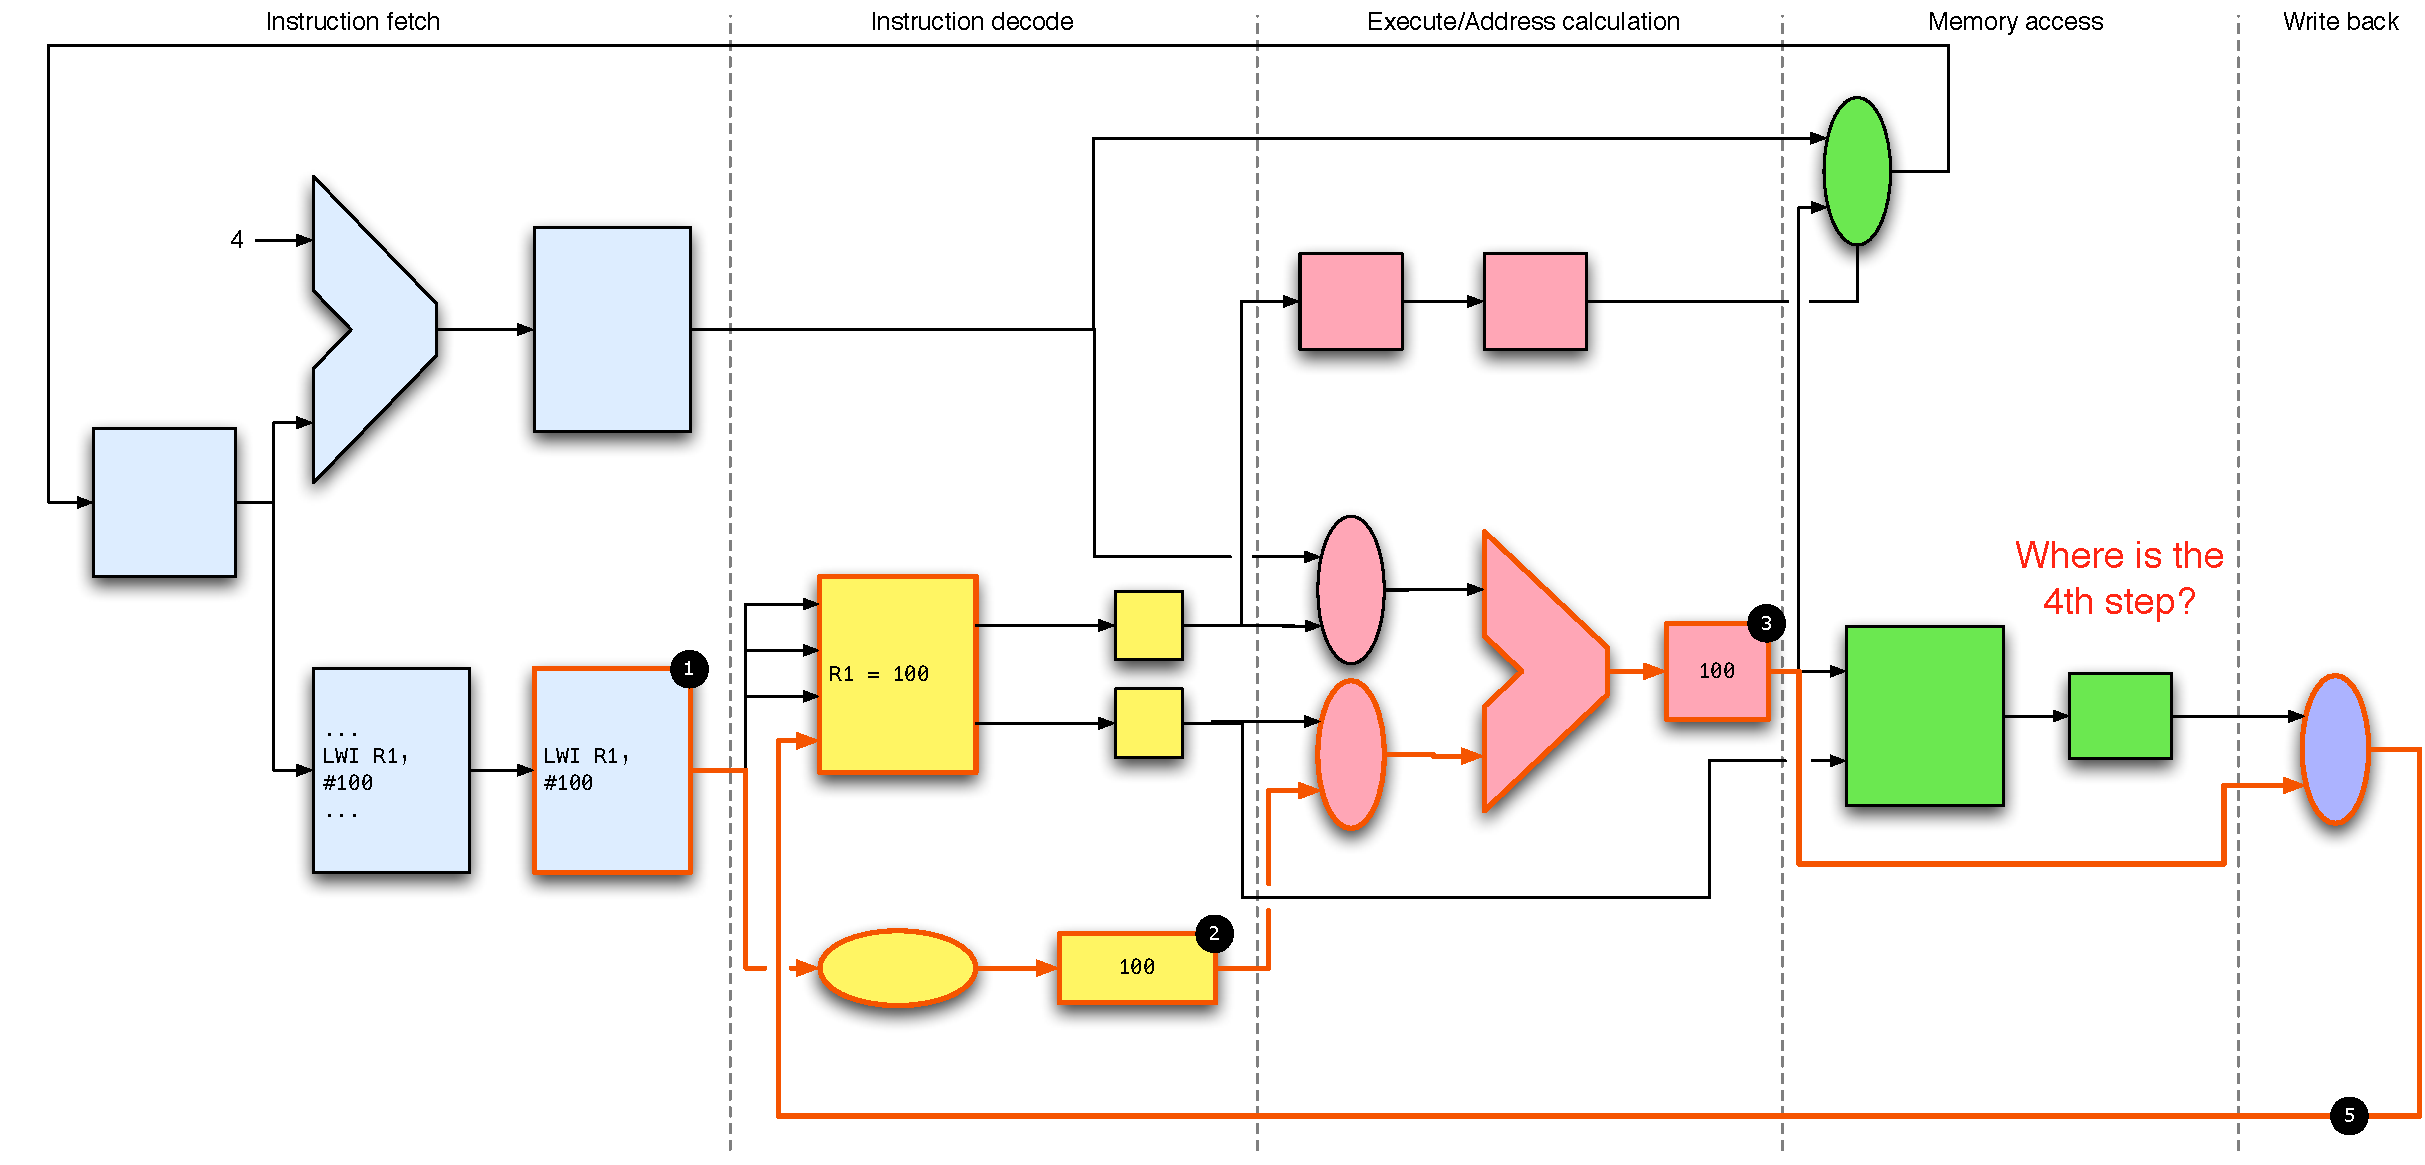
\includegraphics[width=1.1\textwidth]{./images/lwi}
		\end{center}

			
		\subsection{SUB R1 , R2, R3}
		\begin{center}
					 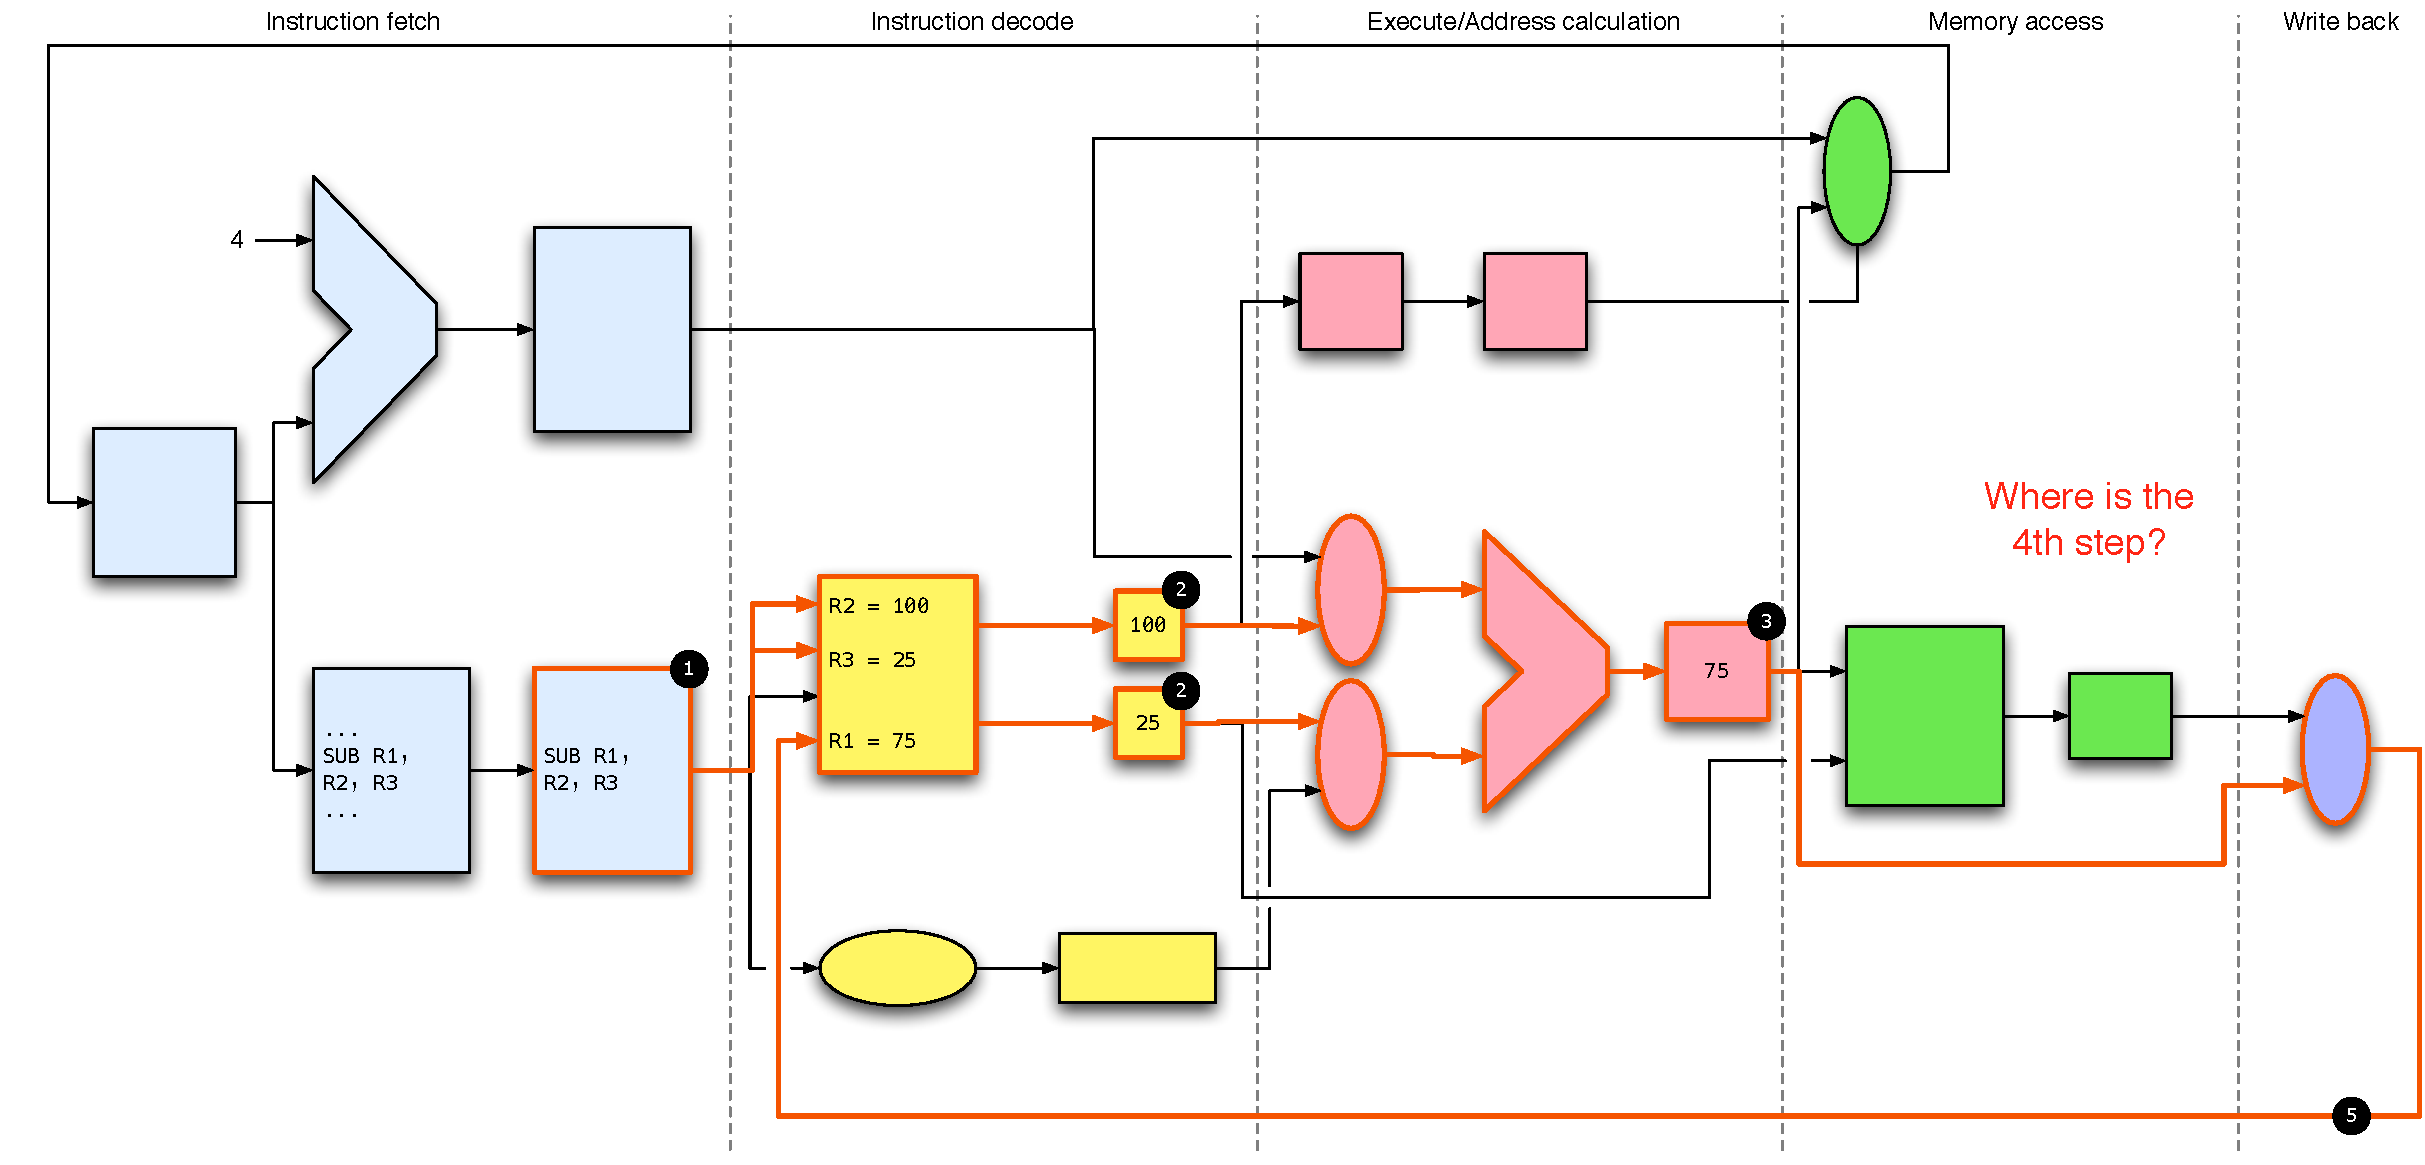
\includegraphics[width=1.1\textwidth]{./images/sub}
		\end{center}

		
		\subsection{SUB R1 , R2, R3}
		\begin{center}
		 			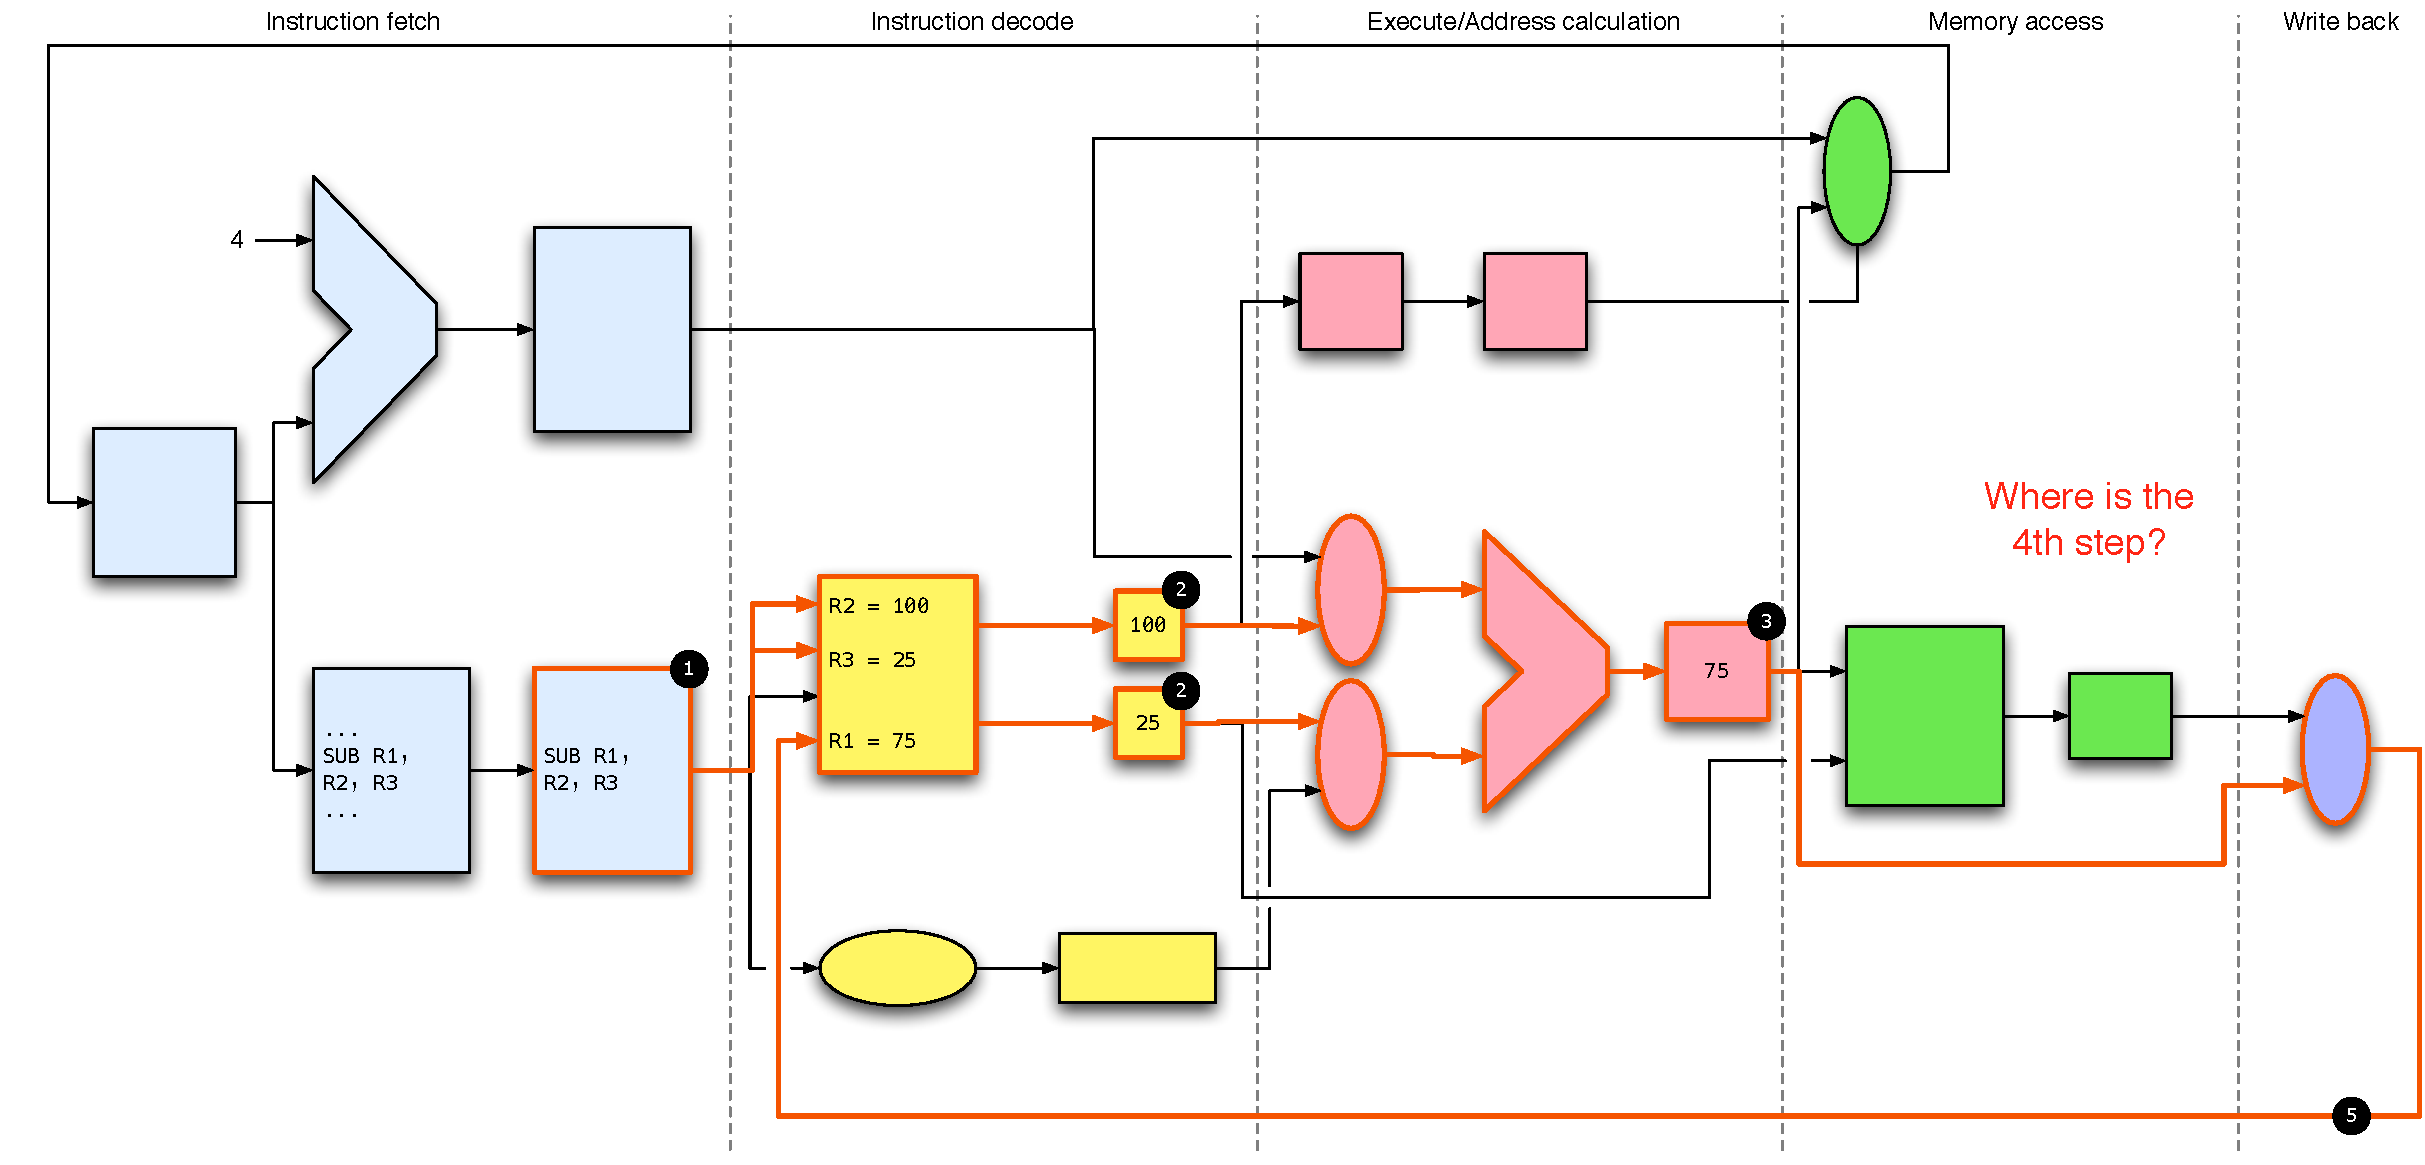
\includegraphics[width=1.1\textwidth]{./images/sub}
		\end{center}
				
			
		\subsection{J test}

		\begin{center}
		 			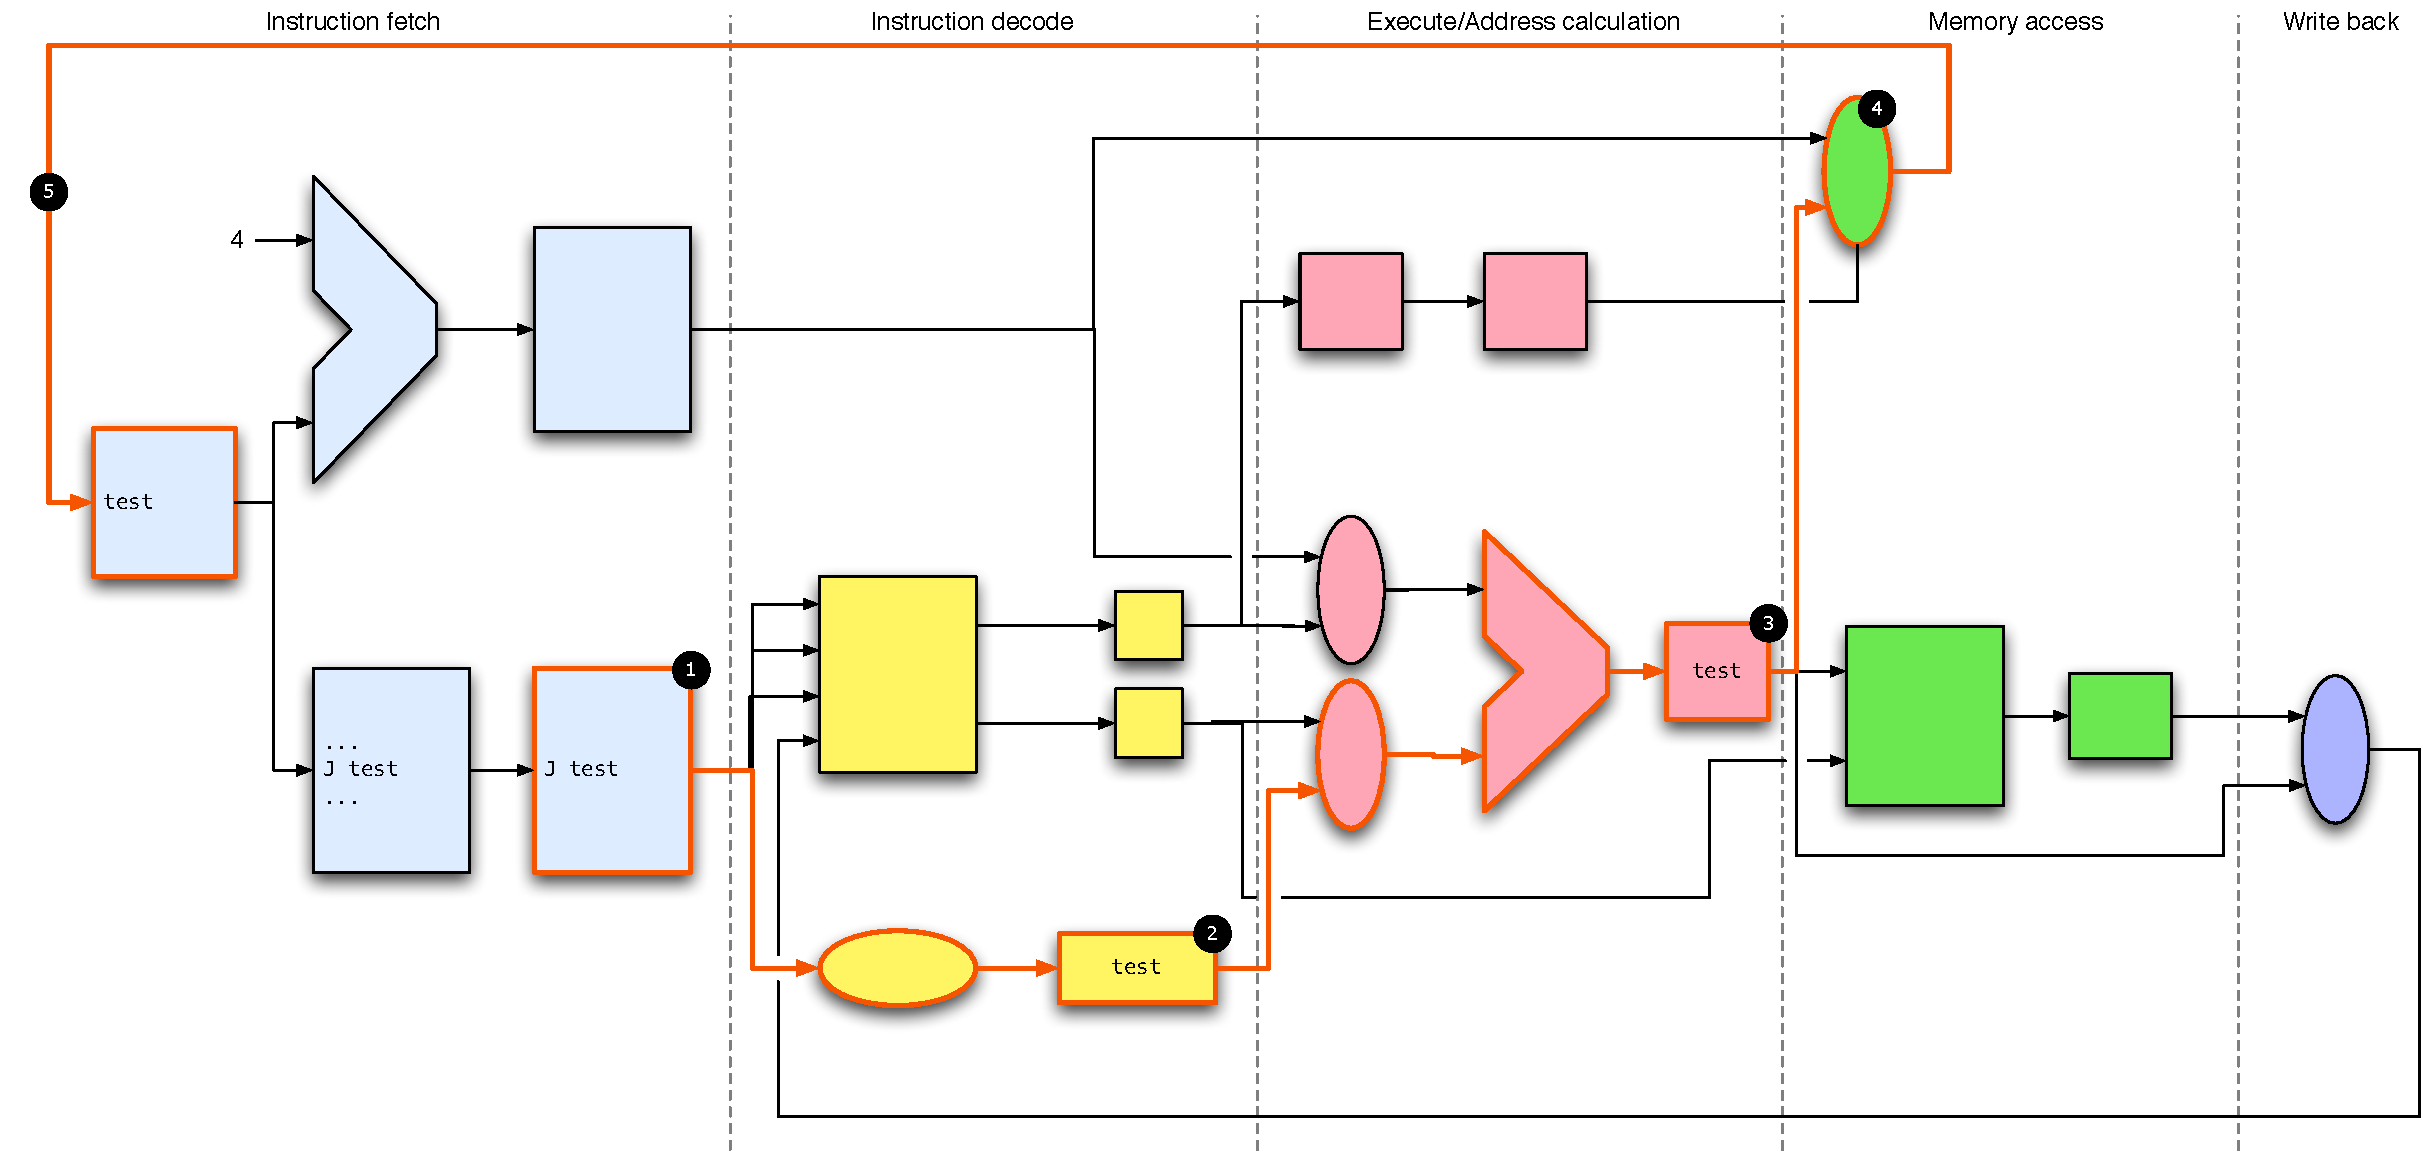
\includegraphics[width=1.1\textwidth]{./images/j}
		\end{center}

			
		\subsection{JR R3}
		\begin{center}
		 			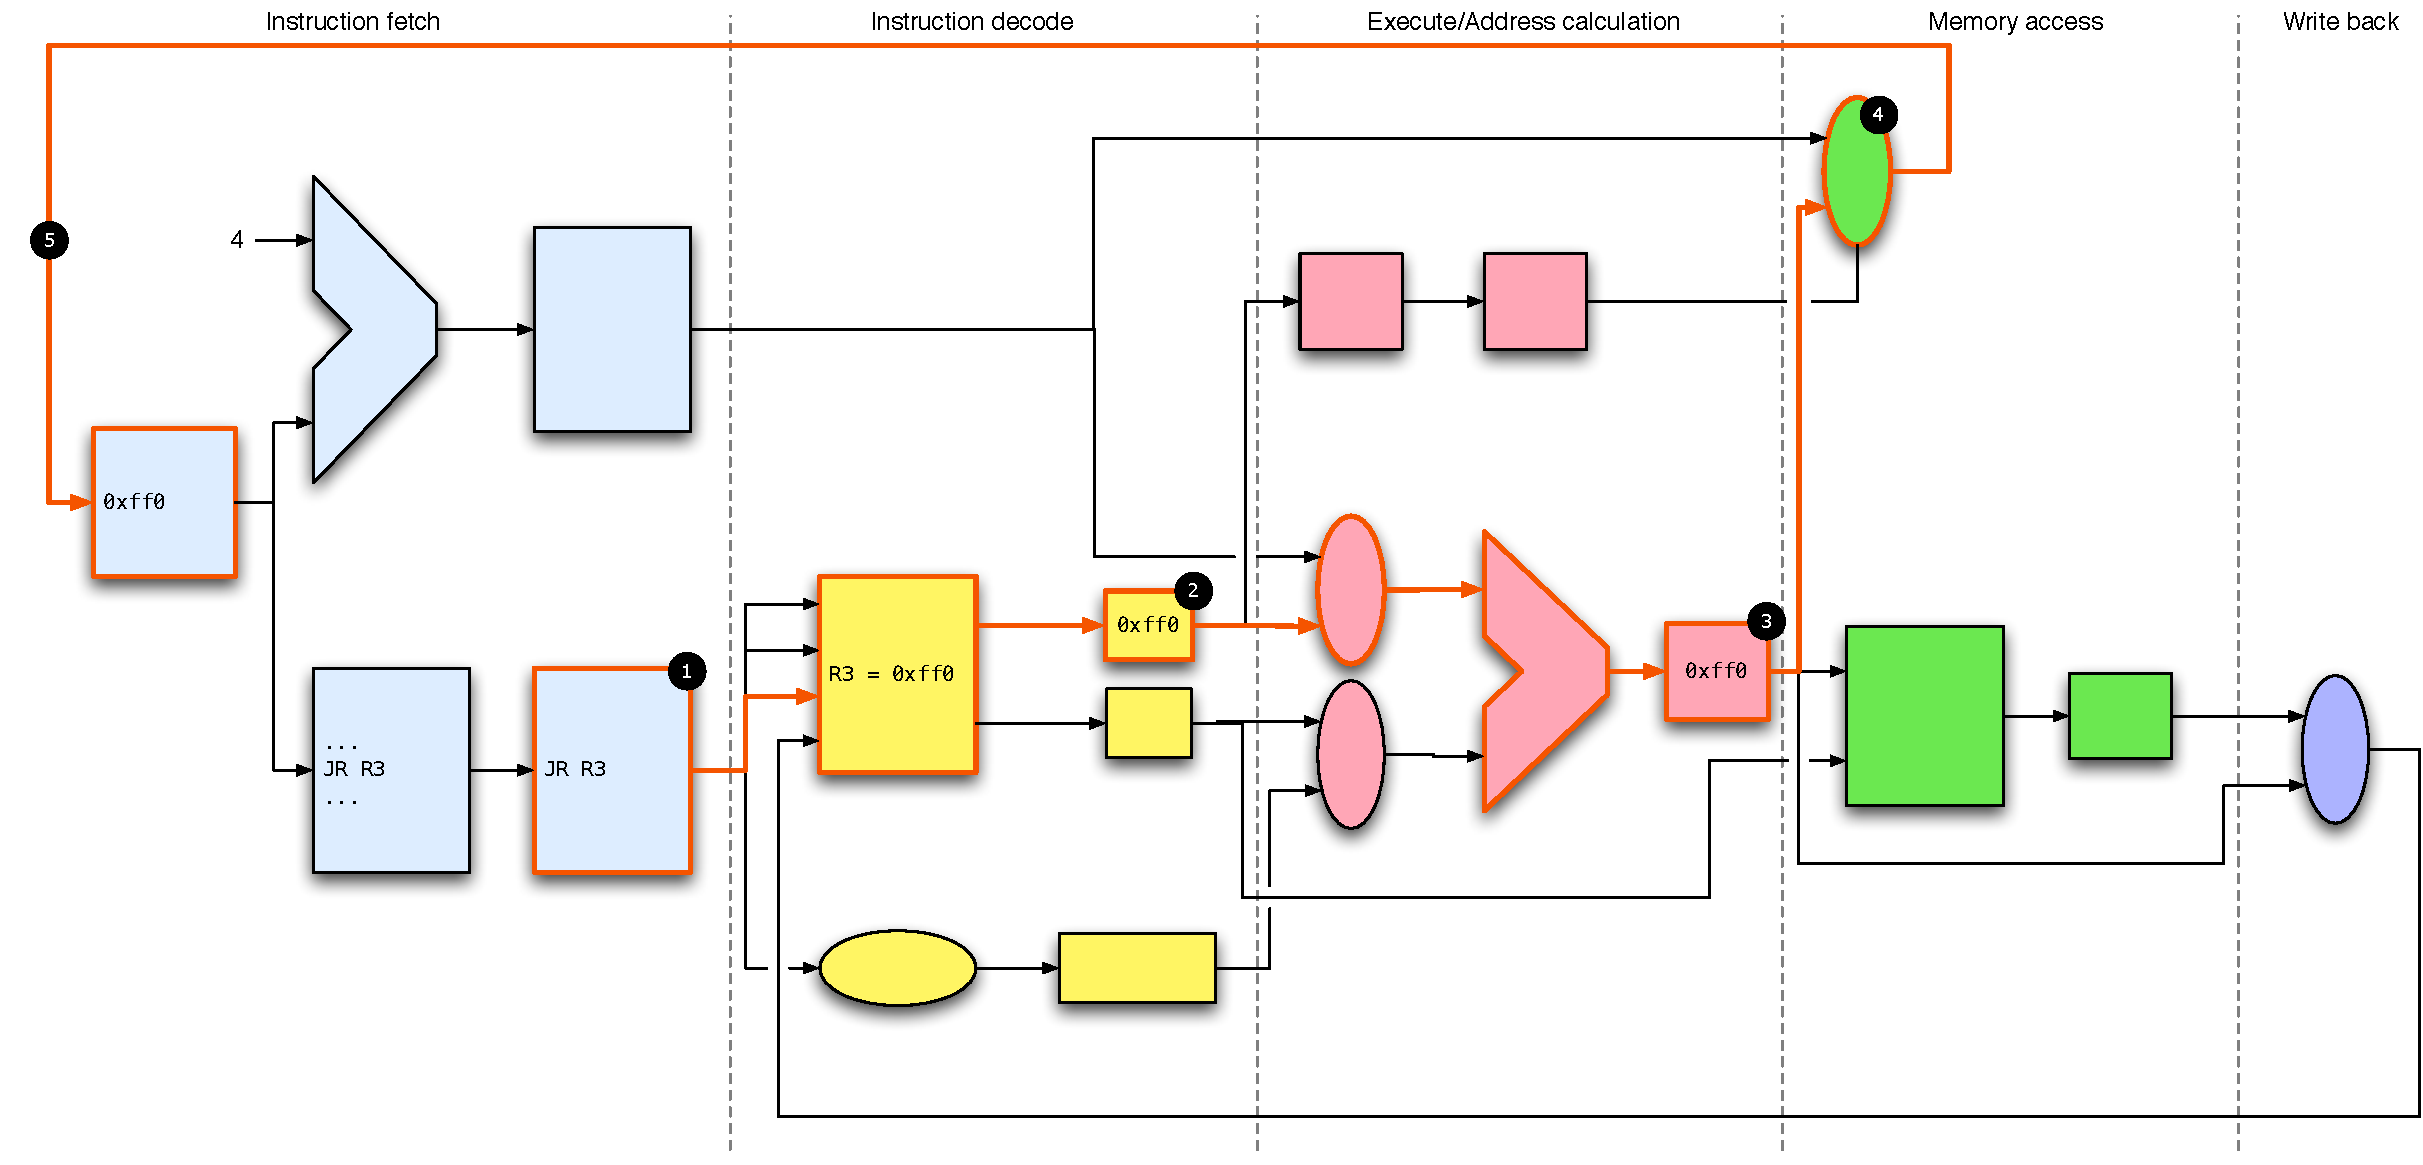
\includegraphics[width=1.1\textwidth]{./images/jr}
		\end{center}

			
		\subsection{BEQZ R4, test}
		\begin{center}
		 			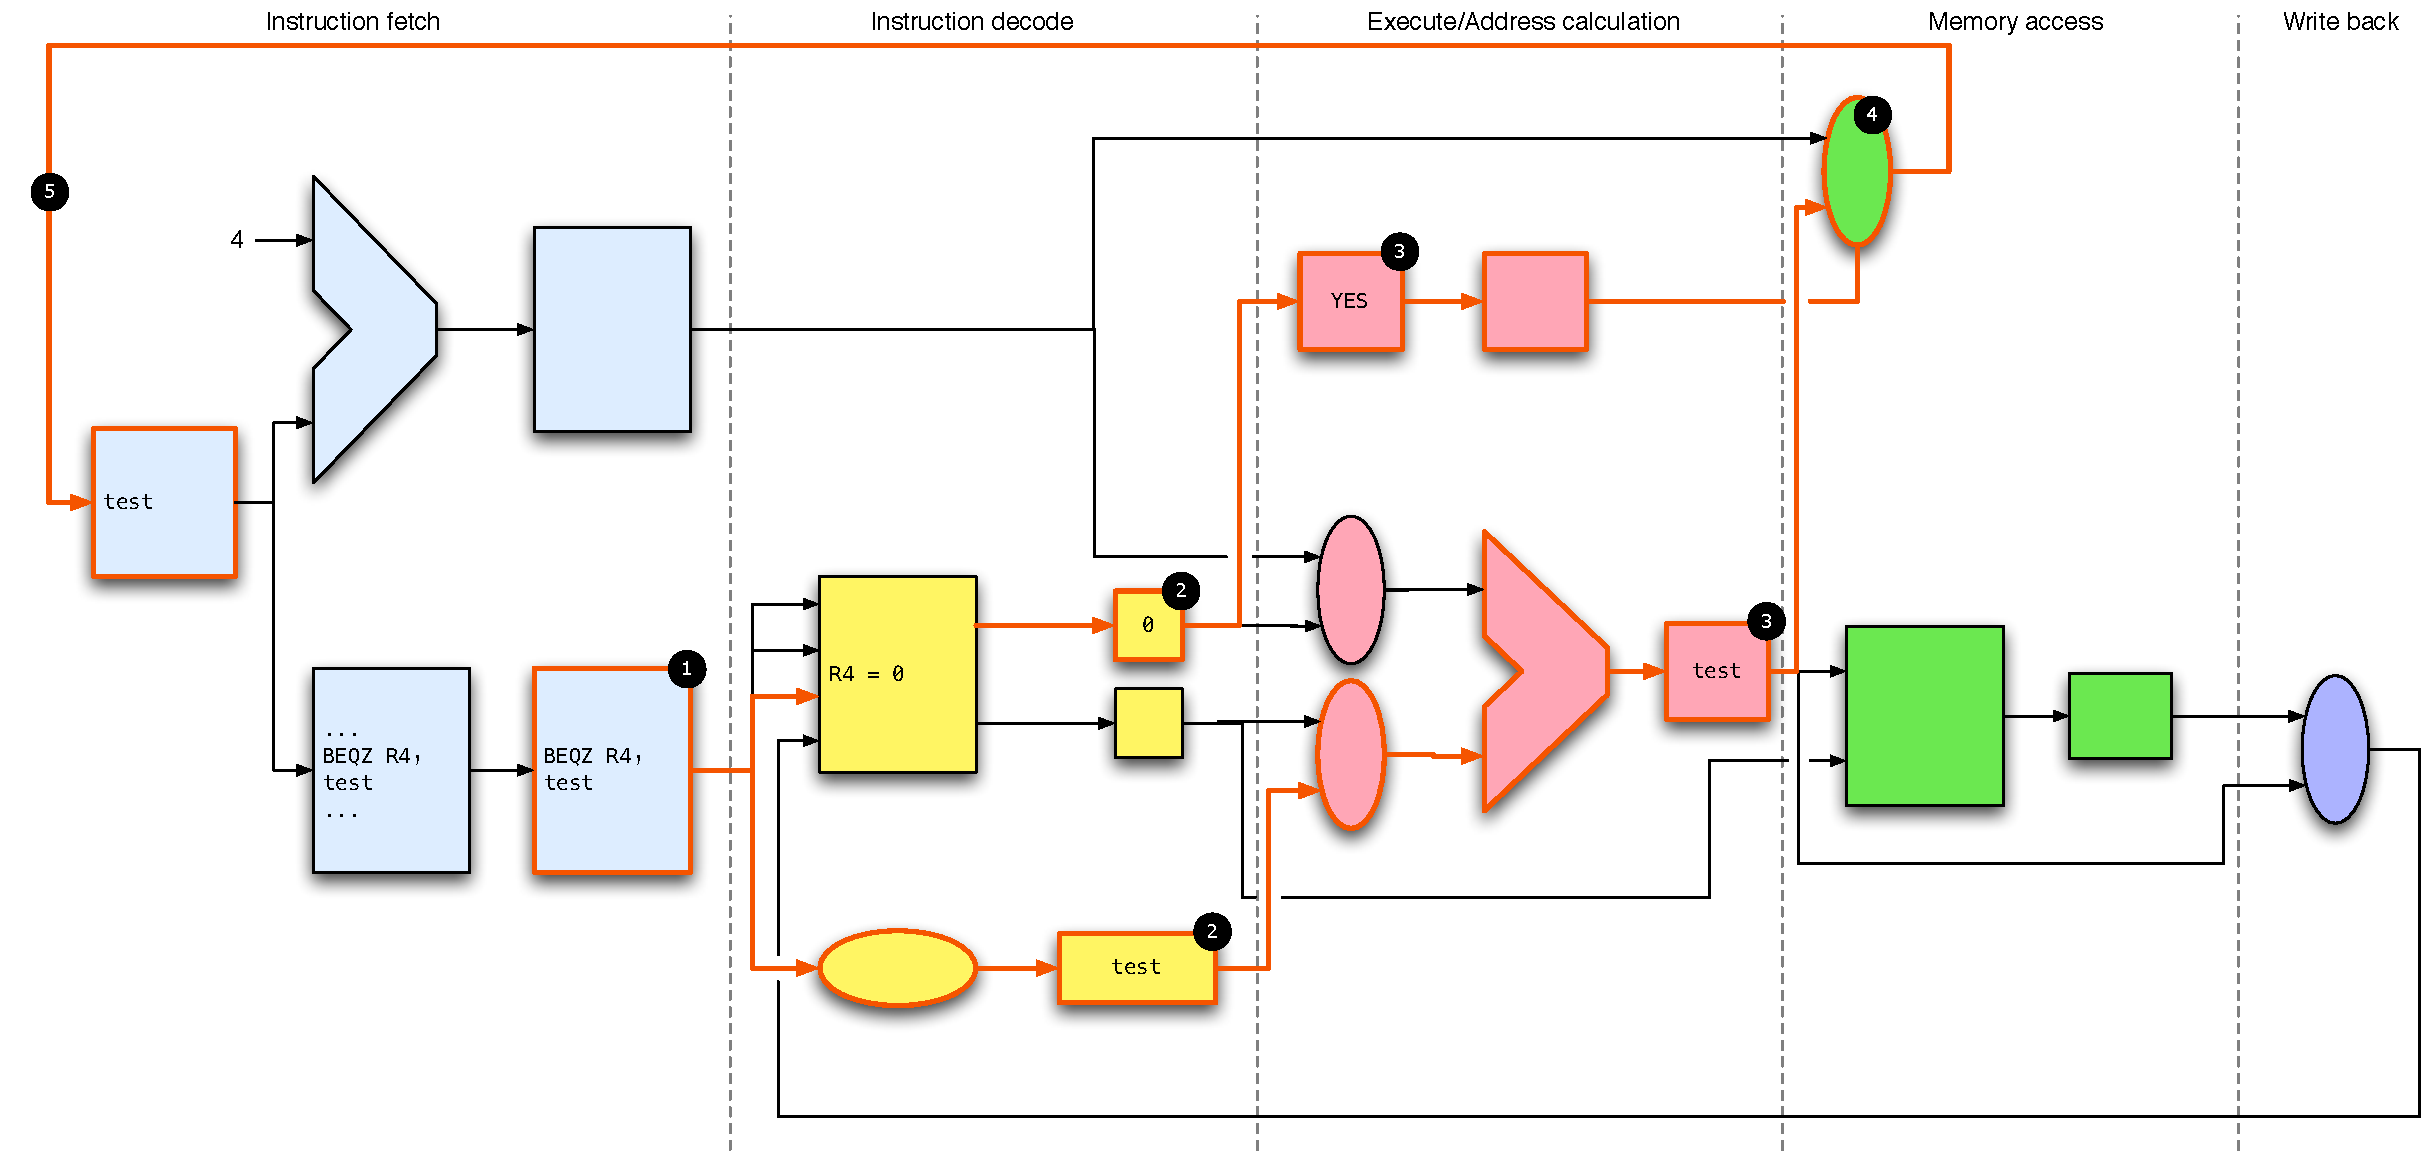
\includegraphics[width=1.1\textwidth]{./images/beqz}
		\end{center}

			
 		\subsection{ADD R1, R2 ,2(R3)}
 			This instruction is not feasible with the architecture(load-store) of this processor. This architecture is allow not to load from 
 			memory directly to the ALU registers 
	\section{ Program,  DLX  processor }
		\subsection{DLX path and hazards }
		\begin{center}
	  		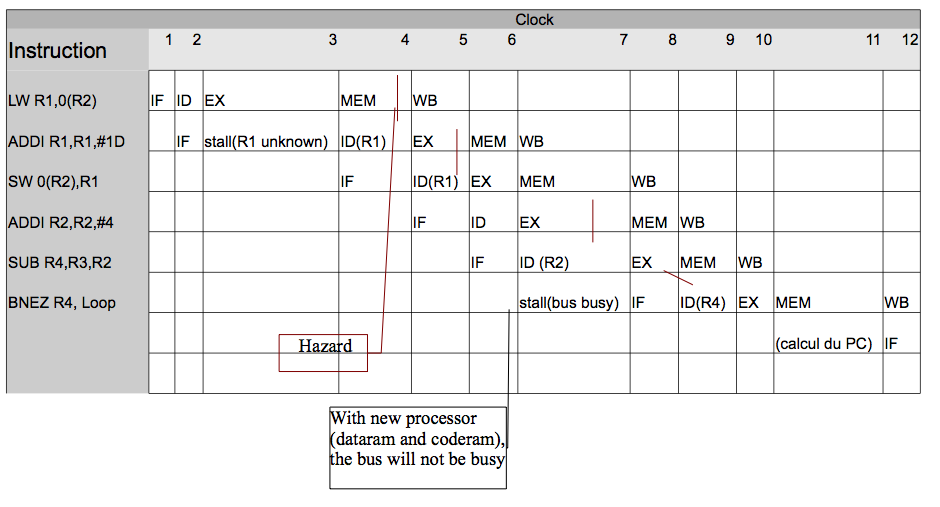
\includegraphics[width=\textwidth]{./images/ex2.png}
		\end{center}
		The hazards are drawn in red.
		
		\section{ Program,  Intel  Processor }
			\subsection{Time measurement}
		\begin{lstlisting} 
static __inline__ unsigned long long rdtsc(void)
{
  unsigned long long int x;
     __asm__ volatile (".byte 0x0f, 0x31" : "=A" (x));
     return x;
}
		\end{lstlisting}
		We have measured the time with this function and the proposed method of this curse . 
		\subsection{Initial program}
				\begin{lstlisting} 
int main(int argc, char * argv[]) {
	int arraySize = atoi(argv[1]);\/\/ The size of the buffer array
	
	int buffer[arraySize];
	
	int ret,j,sum;
	long long t1, t2, t1ms;
	int which = PRIO_PROCESS;
	id_t pid;
	int oldPriority;
	int priority;
	
	pid = getpid();
	oldPriority = getpriority(which, pid);
	priority = -20;
	ret = setpriority(which, pid, priority);
	
	t1 = rdtsc();
	sleep(1);
	t2 = rdtsc();
	
	t1ms = (t2 - t1) / 1000L;
	
	t1 = rdtsc();

	for (j = 0; j < arraySize; j++) {
		sum+=buffer[j];
	}
	
	t2 = rdtsc();
	
	printf(" - Initial:    delta t = %lld [ms]\n", (t2 - t1) / t1ms);
	
	ret = setpriority(which, pid, oldPriority);
	return 0;
}
				\end{lstlisting}
		\subsection{First optimisation program}
				\begin{lstlisting} 
int main(int argc, char * argv[]) {
	int arraySize = atoi(argv[1]);\/\/ The size of the buffer array
	
	int buffer[arraySize];
	
	int ret,j,sum,a,b,c,d;
	long long t1, t2, t1ms;
	int which = PRIO_PROCESS;
	id_t pid;
	int oldPriority;
	int priority;
	
	pid = getpid();
	oldPriority = getpriority(which, pid);
	priority = -20;
	ret = setpriority(which, pid, priority);
	
	t1 = rdtsc();
	sleep(1);
	t2 = rdtsc();
	
	t1ms = (t2 - t1) / 1000L;
	
	t1 = rdtsc();

	for (a=0,b=0,c=0,d=0,j = 0; j < arraySize; j+=4) {
		a+=buffer[j];
		b+=buffer[j+1];
		c+=buffer[j+2];
		d+=buffer[j+3];
	}
	sum = a+b+c+d;
	t2 = rdtsc();
	
	printf(" - firstOptimisation:    delta t = %lld [ms]\n", (t2 - t1) / t1ms);
	
	ret = setpriority(which, pid, oldPriority);
	return 0;
}
				\end{lstlisting}

\subsection{Second optimisation program}
				\begin{lstlisting} 
int main(int argc, char * argv[]) { 	
	int arraySize = atoi(argv[1]);\/\/ The size of the buffer array
	int buffer[arraySize];
	int ret,j,sum,a,b,c,d,e,f,g,h;
	long long t1, t2, t1ms;
	int which = PRIO_PROCESS;
	id_t pid;
	int oldPriority;
	int priority;
	
	pid = getpid();
	oldPriority = getpriority(which, pid);
	priority = -20;
	ret = setpriority(which, pid, priority);
	
	t1 = rdtsc();
	sleep(1);
	t2 = rdtsc();
	
	t1ms = (t2 - t1) / 1000L;
	
	t1 = rdtsc();

	for (a=0,b=0,c=0,d=0,e=0,f=0,g=0,j = 0; j < arraySize; j+=7) {
		a+=buffer[j];
		b+=buffer[j+1];
		c+=buffer[j+2];
		d+=buffer[j+3];
		e+=buffer[j+4];
		f+=buffer[j+5];
		g+=buffer[j+6];
	}
	sum = a+b+c+d+e+f+g;
	t2 = rdtsc();
	
	printf(" - secondOptimisation:   delta t = %lld [ms]\n", (t2 - t1) / t1ms);
	
	ret = setpriority(which, pid, oldPriority);
	return 0;
}
				\end{lstlisting}
				
				
				\subsection{Third optimisation program}

				
								\begin{lstlisting} 

int main(int argc, char * argv[]) {
    int arraySize = atoi(argv[1]);\/\/ The size of the buffer array
	
	int buffer[arraySize];
	
	int ret,j,sum,a,b,c,d,e,f,g,h;
	long long t1, t2, t1ms;
	int which = PRIO_PROCESS;
	id_t pid;
	int oldPriority;
	int priority;
	
	pid = getpid();
	oldPriority = getpriority(which, pid);
	priority = -20;
	ret = setpriority(which, pid, priority);
	
	t1 = rdtsc();
	sleep(1);
	t2 = rdtsc();
	
	t1ms = (t2 - t1) / 1000L;
	
	t1 = rdtsc();
	for (a=0,b=0,c=0,d=0,e=0,f=0,g=0,j = 0; j < arraySize; j+=29) {
		a+=buffer[j];
		b+=buffer[j+1];
		c+=buffer[j+2];
		d+=buffer[j+3];
		e+=buffer[j+4];
		f+=buffer[j+5];

		g+=buffer[j+6];
		a+=buffer[j+7];
		b+=buffer[j+8];
		c+=buffer[j+9];
		d+=buffer[j+10];
		e+=buffer[j+11];
		f+=buffer[j+12];
		g+=buffer[j+13];

		a+=buffer[j+14];
		b+=buffer[j+15];
		c+=buffer[j+16];
		d+=buffer[j+17];
		e+=buffer[j+18];
		f+=buffer[j+19];
		g+=buffer[j+21];

		a+=buffer[j+22];
		b+=buffer[j+23];
		c+=buffer[j+24];
		d+=buffer[j+25];
		e+=buffer[j+26];
		f+=buffer[j+27];
		g+=buffer[j+28];
	}
	
	sum = a+b+c+d+e+f+g;
	t2 = rdtsc();
	
	printf(" - thirdOptimisation:    delta t = %lld [ms]\n", (t2 - t1) / t1ms);
	
	ret = setpriority(which, pid, oldPriority);
	return 0;
}
\end{lstlisting}

	\subsection{MakeFile}
								\begin{lstlisting} 

ARRAY_SIZE=400000000

initial: initial.c
	gcc initial.c -o initial

firstOptimisation: firstOptimisation.c
	gcc firstOptimisation.c -o firstOptimisation

secondOptimisation: secondOptimisation.c
	gcc secondOptimisation.c -o secondOptimisation

thirdOptimisation: thirdOptimisation.c
	gcc thirdOptimisation.c -o thirdOptimisation

timeit: initial firstOptimisation secondOptimisation thirdOptimisation
	@echo Timing a array for an array of $(ARRAY_SIZE) int:
	@./initial $(ARRAY_SIZE)
	@./firstOptimisation $(ARRAY_SIZE)
	@./secondOptimisation $(ARRAY_SIZE)
	@./thirdOptimisation $(ARRAY_SIZE)

clean:
	rm -f initial firstOptimisation secondOptimisation thirdOptimisation
	\end{lstlisting}
	

	
		\subsection{Result}
\begin{lstlisting} 
	Timing a the execution for an array of 400000000 int:
	 - Initial:    delta t = 2216 [ms]
	 - firstOptimisation:    delta t = 1340 [ms]
	 - secondOptimisation:   delta t = 1288 [ms]
	 - thirdOptimisation:    delta t = 1084 [ms]
	 	\end{lstlisting}
	
	


				
\end{document}